\section{Integration of 5G system with non-3GPP access networks}\label{sec:integracao}

Although 5G networks have been designed to serve a wide variety of services, offering a board range of resources, 3GPP envisaged in Release 15 the integration and support of other non-3GPP wireless access technologies, with particular attention to WiFi (IEEE 802.11). As already discussed in some investigations \cite{parkvall2017nr}, \cite{ghosh20195g}, the coexistence of different access technologies promotes significant gains concerning the performance and cost of the communication of IoT devices. Moreover, many devices have a non-3GPP wireless interface, and these devices will be in operation for some years. The integration of multiple wireless access technologies in an only core can benefit both users and administrators of public and private communication infrastructure.

Release 15~\cite{3GPP:19} already defines how non-3GPP wireless network technology can be used as access and integrated into a 5G core. However, this release focus only on Wireless Local Area Networks (WLANs), \textit{i.e.}, WiFi networks, considering the untrusted access. The trusted access will be introduced in Release 16~\cite{WBA-NGMN:19}. In this release, attention is also being taken to cable access technologies, in particular for HFC. Although 3GPP standards do not explicitly describe how to integrate other wireless communication technologies used in IoT, such as LoRa and ZigBee, the framework allows extensions to be exploited~\cite{navarro-ortiz:18,yasmin:17}. In the following, we present more details about Release 15 and also on LoRa/LoRaWAN technology, which we use as an illustration for the integration between the 5G core and a non-3GPP wireless access technology at the end of this section.


\subsection{Non-3GPP Access Networks}\label{subsec:nao-3GPP}
 
The 5G core architecture foresees, since its design, the possibility of integrating non-3GPP access technologies, with the premise that the communication interfaces offer IP connectivity, \textit{i.e.}, a traditional IP stack. Although this premise is met for technologies such as WiFi and HFC, several IoT solutions such as LoRa, ZigBee, nRF24, and others consider that exists a gateway to provide the IP connectivity for the IoT devices. Therefore, we assume from this point in the article that equipment with a traditional IP stack, \textit{i.e.}, a device or a gateway, is available to establish the integration with the non-3GPP network. It is essential to highlight, as describe by~\cite{yasmin:17} that there are several ways to integrate devices that depend on a gateway with a traditional IP stack.

The EPC core from 4G also has support for the non-3GPP access network, using a more sophisticated approach. Moreover, for defining between trusted and untrusted access, it needs to choose between network-based mobility and host-based mobility. Considering the focus of this article, no further information on the EPC core approach will be present, but a full description can be found in~\cite{olsson:13}. For the 5G SBA core, fewer options were defined, basically, \textbf{untrusted} non-3GPP access (Release 15, frozen in March 2019 and completed in June 2019) and \textbf{trust} (Release 16, expected to freeze in March 2020 and conclusion to June 2020). In this context, the term untrusted means that the 3GPP network operator does not trust in the security offered by the non-3GPP access network. Therefore, it needs to take actions that ensure the proper transport of traffic from this access network. This need means that the non-3GPP traffic must be isolated from other traffics, including the 5G core, which is suitable for IoT applications and services. The trust access does not allow integration with other wireless communication technologies used in IoT, such as LoRa or ZigBee.

To support the untrusted non-3GPP access network, the main component introduced by 3GPP Release 15 was N3IWF, which is responsible for forwarding signaling and data between the 5G core and the non-3GPP access network, as described in Subsection \ref{sec:core}. Fig.~\ref{fig:non3gpp_untrusted} illustrates the integration of two non-3GPP access networks to a 5G core, showing the main components involved and their communication interfaces. N3IWF selects AMF to serve the IoT device (or gateway), which will be responsible for holding the (eventual) mobility of the equipment and brokering all the signaling with other 5G core functions. For effective communication, a device needs PDU sessions, which are established, modified, and released under the SMF component's control. This component works as a CP that operates on a DP implemented through the UPF component.

\begin{figure}[htb]
 \begin{center}
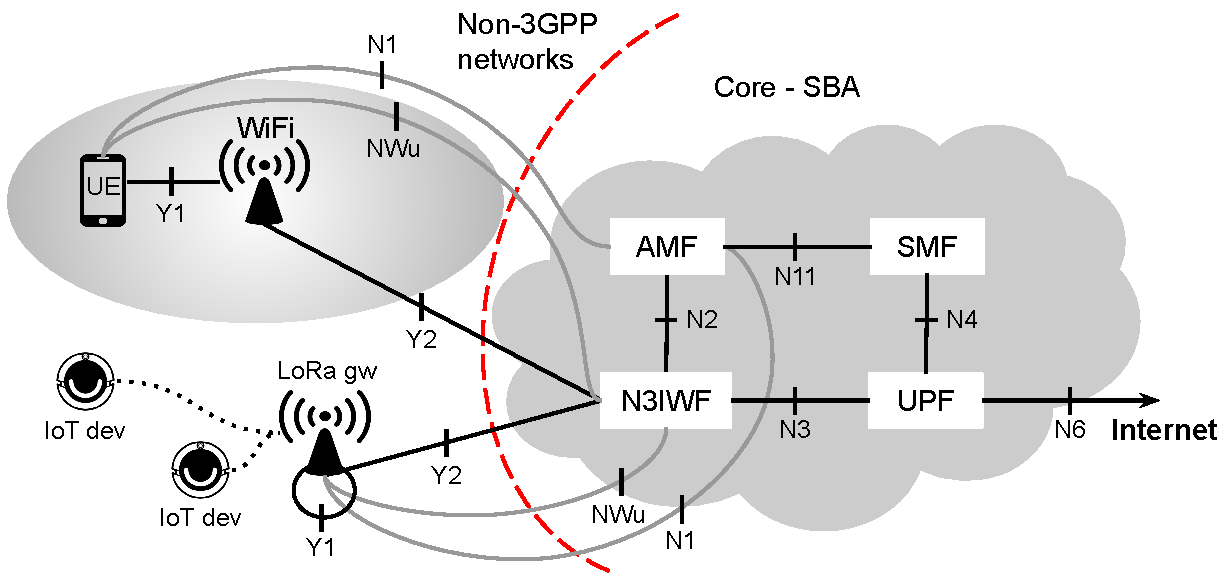
\includegraphics[width=0.5\textwidth]{figs/non3GPP_untrusted.pdf}
  \end{center}
\caption{Integration between the untrusted non-3GGP access networks and the 5G SBA core.}
\label{fig:non3gpp_untrusted}
\end{figure}

In the 5G SBA core, the AUSF component allows a device to authenticate itself to access the network and its services using a 3GPP wireless interface (\textit{e.g.}, NR) and a non-3GPP interface (\textit{e.g.}, WiFi). Non-3GPP devices can authenticate with the SBA core through a certification-based scheme, using Extensible Authentication Protocol-Transport Layer Security (EAP-TLS) or EAP-Tunneled TLS (EAP-TTLS) and the traditional procedure with credentials based on Subscriber Identification Module (SIM). Fig.~\ref{fig:non3gpp_connections} shows the connections established to provide integration between the untrusted non-3GPP access network and the 5G SBA core.

\begin{figure}[htb]
 \begin{center}
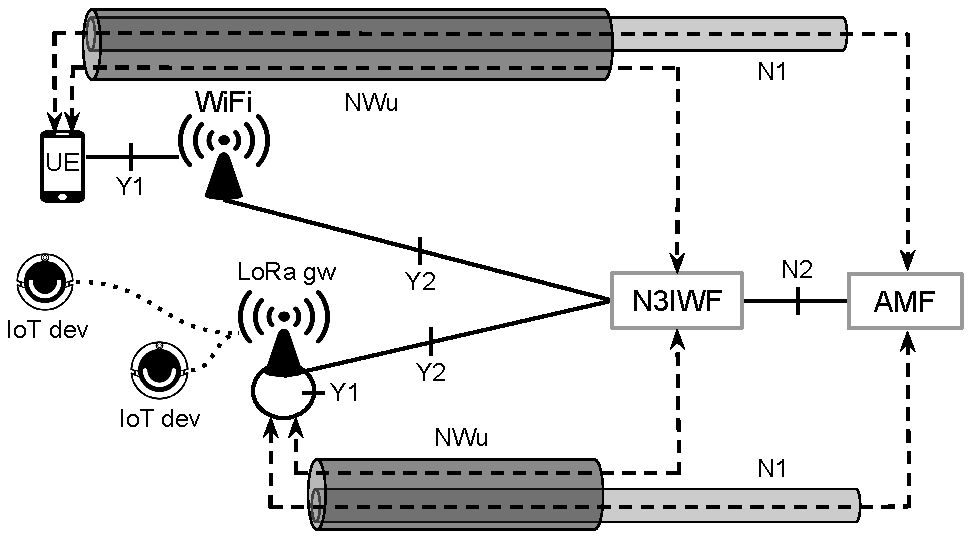
\includegraphics[width=0.5\textwidth]{figs/non3GPP_connections.pdf}
  \end{center}
\caption{Connections for the integration of untrusted non-3GPP access network with the 5G SBA core.}  
%\caption{Conexões para a integração de redes de acesso não-3GPP não-confiável com o núcleo SBA da 5G.}
\label{fig:non3gpp_connections}
\end{figure}


3GGP does not define the Y1 connection, but this connection establishes the communication of the device with its access network, \textit{e.g.}, through a WiFi access point or LoRa gateway. It is assumed that there is some authorization process through the Y1 connection, allowing the device to access the network and to obtain an IP address. However, several technologies, such as LoRa, do not directly assign IP to the devices, and part of the Y1 connection needs to be implemented at the technology gateway itself. The Y2 connection is also not defined by 3GPP, but it must provide communication between the access network and the N3IWF component of the SBA core. This connection can be established in almost any way, including via the public Internet, \textit{i.e.}, potentially with multiple equipment and intermediate technologies.

The 3GPP standard specifies that between the device (or gateway) and the N3IWF component, an encrypted IPSec tunnel, called NWu, must be established for sending data and signaling traffic. N3IWF selects AMF to serve the device, and the N2 interface between the two functions is established. After setting NWu and N2, the 3GPP standard specifies that it is possible to create the N1 interface between devices (or gateway) and the AMF component for transporting Non-Access Stratum (NAS) signaling. This approach differs from that used in the 4G EPC core, in which NAS signaling applies only to 3GPP access networks. In the 5G SBA core, devices connected via non-3GPP access networks are managed similarly to devices connecting via 3GPP access networks.


\subsection{LoRa}

LoRa technology, developed by Semtech Corporation~\cite{semtech}, allows communication over long distances using the Spread Spectrum concept of RF. This technology has the following configuration parameters that directly influence the communication performance:

\begin{itemize}
\item Spreading Factor (SF) with values of 7, 8, 9, or 10. The higher SF, more information is transmitted per symbol, generating a gain in transmission;
\item Bandwidth (BW) of 125 kHz, 250 kHz, or 500 kHz for a given SF. A narrower BW increases the reception sensibility and increases the packet transmission time;
\item Code Rate (CR) is responsible for detecting and correcting errors.
\end{itemize}

These configurations determine the bit rate transmitted, the maximum size of the transmitted data, and the transmission time of a packet in the RF spectrum. These configurations also influence the size of messages, their range, and the energy consumption of the IoT device.

According to ~\cite{shanmuga2020} and ~\cite{Lee2017}, Lora is resistant to interference, due to its wide range of SFs, which can be used in urban, rural, and even industrial environments. Moreover, this technology offers four times the coverage range, compared to other radio technologies due to its robust nature and ability to work with low-intensity radio signals. Its ability to perform multiple transmissions on the same RF channel, with the use of different SFs, reduces the likelihood of collisions, increasing the effective data transmission rate, allowing discrimination between time and frequency errors. Therefore, LoRa is considered one of the most promising technologies for the physical layer of sensor networks and, consequently, for IoT~\cite{Haxhibeqiri2018}. However, to have a useful application of sensors and IoT, it is necessary to have a network, such as LoRaWAN, described below.


\subsection{LoRaWAN network}

LoRaWAN network is the name given to IoT Low Power Wide Area Network (LPWAN), which uses the LoRa technology as a physical medium and implement an architecture based on the LoRaWAN Media Access Control (MAC) protocol. In Fig.~\ref{fig:mac_lorawan}, we can see the MAC layer, its sublayers, and the LoRa physical layer, enabling the long-range communication link.  The MAC layer protocol and the network architecture have a significant influence on determining the battery life a sensor, network capacity, QoS, security, and the range of IoT applications served.


\begin{figure}[!h]
 \begin{center}
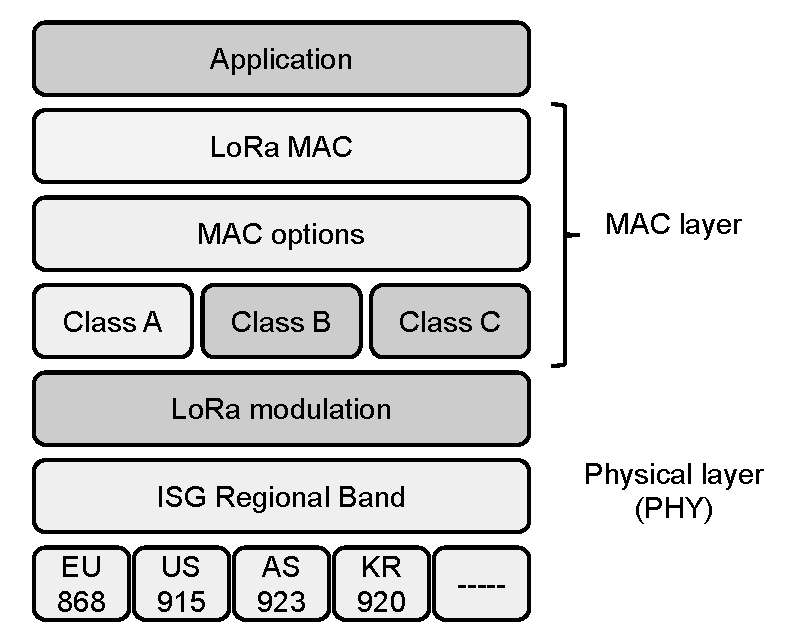
\includegraphics[width=0.45\textwidth]{figs/mac_lorawan-2.pdf}
  \end{center}
\caption{LoRaWAN architecture layers.}
\label{fig:mac_lorawan}
\end{figure}

The LoRaWAN protocol is based on open, low-cost standards. This protocol was designed from the beginning to implement platforms for IoT. In this way, the scope of supported IoT applications is broad, making this technology attractive to the 5G system and creating an IoT network with a large coverage area. Among the possible uses, there are smart grids for electrical energy, sensor networks of several types, precision agriculture, and others.


Fig.~\ref{fig:topologia_lorawan} shows the LoRWAN protocol reference topology. A prominent feature of this technology is its low energy consumption, due to the star topology that does not require routing between nodes. The central component is the LoRaWAN gateway that can be connected to a 5G system on untrusted non-3GPP access. These gateways, also known as concentrators, have models that can meet specific demands, simpler and cheaper for closed environments, in contrast to industrial models with protection against the weather and external applications. In communication between gateway and devices, there are two previous types of messages exchange: Unconfirmed Data Message, similar User Datagram Protocol (UDP) messages, and Confirmed Data Message, like to Transmission Control Protocol (TCP). Another fundamental characteristic of the LoRaWAN network is the existence of three devices classes that communicate with the gateways, which are described in the following.

\begin{figure}[!h]
 \begin{center}
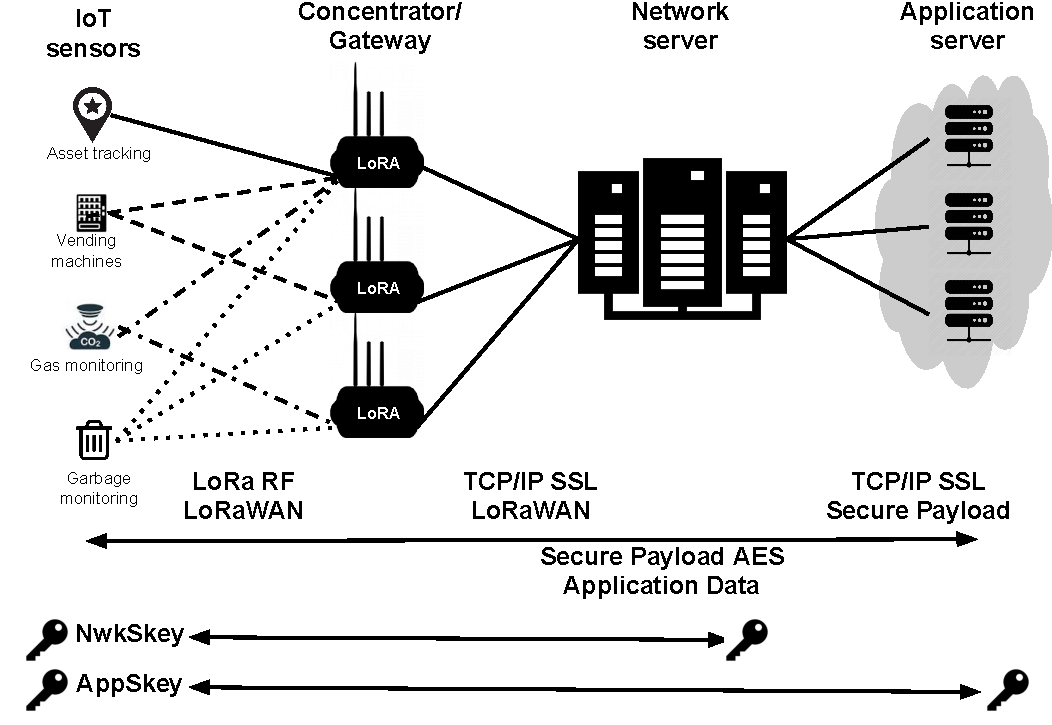
\includegraphics[width=0.5\textwidth]{figs/topologia_lorawan-2.pdf}
  \end{center}
\caption{LoRaWAN network topology}  
\label{fig:topologia_lorawan}
\end{figure}


\begin{itemize}
\item Class A: upstream transmissions (device-gateway) are based on the ALOHA protocol. The reception of the can only be performed in two short reception windows that open after a transmission. This class provides the lowest energy consumption, with the main application of the monitoring quantities.
\item Class B: in addition to the class A mode, pre-programmed transmission windows (gateway-device) and managed by a timing signal (Beacon) are opened, which indicates when the receiver is ready to receive the signal. This class can be convenient for remote control systems that are not time-sensitive.
\item Class C: the transmission window (gateway-device) is open continuously, closing only at the time of the upstream transmission (device-gateway).
\end{itemize}

Regarding the activation of devices on the network, LoRaWAN adopts the AES-128 encryption algorithm, using two different forms of activation due to the Public or Private network. In public networks, it uses Over The Air Activation (OTAA), which is based on sending a unique global identifier (DevEUI), analogous to the MAC address, identifier (AppEUI) and application key (AppKey) desired. This data is used in the application layer to validate and activate it in a given network application. After the acceptance on the network, the device receives a message \texttt{join accept}, which has the device address (DevAddr), the network session key (NwkSKey), and the application session key (AppSKey). In private networks, the following data are required for activation: device address (DevAddr), network session key (NwkSKey), and application session key (AppSKey), which are recorded on the device, at the time of configuration. Therefore, the device is ready for communication when it is connected to the network.

In the LoRaWAN architecture, Network Servers are still responsible for managing the information sent by gateways. As there is the possibility that two or more gateways receive the same packet from a given device, the network server eliminates duplicate packets, manages the acknowledgment (ACK) return times, and makes the adjustments for the adaptative data rate to manage the times between communications and energy consumption. Finally, LoRaWAN has one or more Application Servers that receive packets from Network Servers via request or automatically and, according to the request, perform one or more specific actions providing the needed interface for various client applications. 

\subsection{Demonstration of the integration of non-3GPP wireless access network and the 5G core} \label{sec:eRAN}

\subsection*{Goals}

The goal of the demonstration is to introduce a non-3GPP wireless access network to the 5G core. Moreover, this experiment shows the great capillarity that the 5G system can have, including network with unlicensed frequencies. 

\subsection*{Description}

In this demonstration, we combine a RAN based on LTE technology with a LoRaWAN wireless network implemented in hardware. For RAN LTE, we use open-source software and an SDR. We also use an open-source implementation of the SBA-based 5G core software. All components are implemented using Docker containers that can be hosted on a cloud infrastructure. Connected to access the network through LTE, there is a LoRaWAN gateway implemented in generic hardware with support to multiples IoT sensors that synchronize its data with the LoRaWAN server present at the other end of the infrastructure. Therefore, for demonstration purposes, the data collected by the sensors are transmitted via the LoRa network to the gateway that forwards the data via LTE backhaul, passing through the SBA core of the 5G network until reaching the LoRaWAN server. Fig.~\ref{fig:demo3} shows the experiment we designed to demonstrate the integration of a non-3GPP wireless access network with a 5G core network.


\begin{figure}[htb] 
 \begin{center}
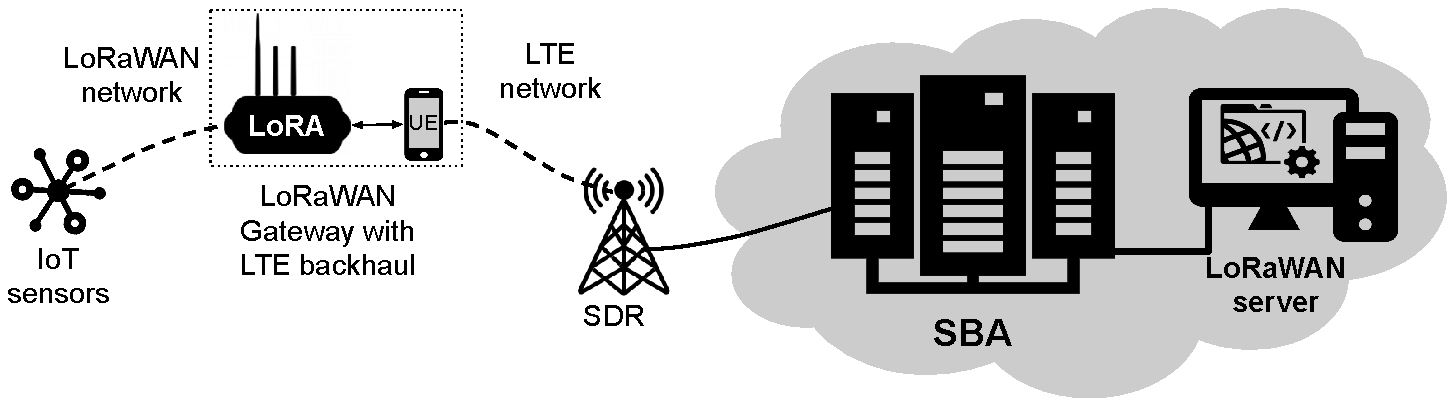
\includegraphics[width=0.5\textwidth]{figs/demo3.pdf}
  \end{center}
\caption{Demonstration of the integration of a 5G core with a non-3GPP access network based on LoRa.}
\label{fig:demo3}
\end{figure}

\subsection*{Additional information}

During the tutorial, we present a demonstration video of the experiment. Moreover, a manual is available with details on how the practices can be replicated. Finally, containers and any extra code produced by the team needed to replicate the experiment is also publicly available.

Repository for this tutorial:\\
\url{https://github.com/LABORA-INF-UFG/NetSoft2020-Tutorial4}.


